\documentclass[conference]{IEEEtran}
%\renewcommand{\thesubsection}{\thesection.\alph{subsection}}
\renewcommand{\floatpagefraction}{.8}%
%\addtolength{\oddsidemargin}{-.875in}
%\addtolength{\evensidemargin}{-.875in}
%\addtolength{\textwidth}{1.75in}
%\addtolength{\topmargin}{-.875in}
%\addtolength{\textheight}{1.75in}
	
\usepackage{bm}
\usepackage{amsmath}
\usepackage{amssymb}
\usepackage{tikz}
\usetikzlibrary{automata,positioning}
\usepackage{url}
\usepackage{float}
\usepackage{setspace}
\usepackage{filecontents,lipsum}
\usepackage[noadjust]{cite}
\usepackage{listings}



\begin{document}
%\raggedright
%\doublespacing

\title{Research Proposal for Code Smell Algorithm Training Dataset Analysis}
\author{Rodger Byrd\\rbyrd2@uccs.edu}
\maketitle

\section{Introduction to the Problem}
A code smell is a description of a pattern in code that might cause deeper problems. 
Code smells are not easily found and can vary by programming language and development methodoligies.
The existence of code smells and antipatterns implies that there are potential problems with software sustainment and imply there are issues with the design.
Kent Beck coined the term ``code smell'' \cite{fowler_refactoring:_2018} and defined as ``certain structures in the code that suggest (sometimes they scream for) the possibility of refactoring''.
Machine learning is defined as computers learning to solve problems without being explicitly programmed, although they are ``trained''\cite{bishop_pattern_2006}. 
Arthur Samuel coined the term Machine Learning in 1959\cite{samuel_studies_1988}.
Machine learning is a subset of artificial intelligence. 
It uses algorithms and statistical models to execute a task without explicitly being programmed.
Machine learning is used in a wide variety of applications such as email spam filtering, search engines, video surveillance, and image curation.
The big challenge in this field seems to be the best way to identify code smells and how training datasets are labeled and created.
There is a lot of inconsistency in training datasets and identifying code smells because they can be subjectively interpreted.
Additionally, expert advice and knowledge may be able to help identify code smells, using it to train datasets may not be effective unless it has been experimentally shown to be result in finding code smells. 

It is difficult to compare the results of previous research due to the variability of training datasets and differences in machine learning algorithms.
This research will compare training datasets and code smell definitions for performance.

Figure \ref{fig:ts} show the "potential" results of comparison by algorithm. 

\begin{figure*}[ht]{
  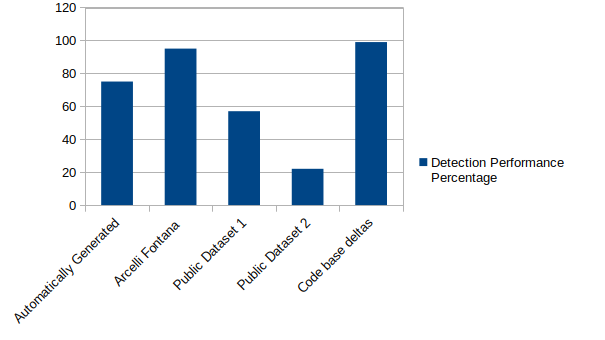
\includegraphics[width=\columnwidth]{teaser.png}}
  \caption{Training Data Performance}
  \label{fig:ts}
\end{figure*} 

\section{The Approach}
The approach to this research will be to compare training datasets for performance in detecting code smells.
Common existing public datasets will be compared using the highest performing algorithms to determine which has the best performance.

\section{Experimental Design}
%A formal section on Experimental Design and datasets 

\section{Hypothesis and Stastical Testing}
%A formal section on the hypothesis and Statistical Testing for that hypothesis for your given design and the outcomes of the experiments.
\subsection{Hypothesis}
Hypothesis 1: Different training datasets will have varying performance
Hypothesis 2: Highest performing datasets can be optimized and improved
\subsection{Stastical Testing}

\section{Research Plan and Timeline}
Beginning Springs 2020 the following milestones will be met:
\begin{enumerate}
\item The commitee for thesis will be identified
\item The research proposal will be presented to the committee for approval.
\item Research will begin
\end{enumerate}

%Relevan papers are referenced in the bibliography below. 
%\nocite{*}
%\clearpage


\bibliographystyle{IEEEtran}
\bibliography{references}


\end{document}